\documentclass[15pt]{beamer}
\usetheme{Warsaw}
\usepackage{enumitem}
\usepackage{multicol}
\usepackage{multirow}
\usepackage{graphics}
\usepackage[export]{adjustbox}
\usepackage{bookmark}
\usepackage{graphicx}


\setbeamercolor{normal text}{fg=white,bg=black!90}
\setbeamercolor{structure}{fg=white}

\setbeamercolor{alerted text}{fg=red!85!black}

\setbeamercolor{item projected}{use=item,fg=black,bg=item.fg!35}

\setbeamercolor*{palette primary}{use=structure,fg=structure.fg}
\setbeamercolor*{palette secondary}{use=structure,fg=structure.fg!95!black}
\setbeamercolor*{palette tertiary}{use=structure,fg=structure.fg!90!black}
\setbeamercolor*{palette quaternary}{use=structure,fg=structure.fg!95!black,bg=black!80}

\setbeamercolor*{framesubtitle}{fg=white}

\setbeamercolor*{block title}{parent=structure,bg=black!60}
\setbeamercolor*{block body}{fg=black,bg=black!10}
\setbeamercolor*{block title alerted}{parent=alerted text,bg=black!15}
\setbeamercolor*{block title example}{parent=example text,bg=black!15}

\addtobeamertemplate{navigation symbols}{}{%
    \usebeamerfont{footline}%
    \usebeamercolor[fg]{footline}%
    \hspace{1em}%
    \insertframenumber/\inserttotalframenumber
}


\title{SPACE INVADERS}


\author[Muttakin \and Numan]{Nurul Muttakin [1305009] \and \\ S. Mahmudul Hasan (Numan) [1305043]}

\institute[BUET]{Bangladesh University of Engineering and Technology}

\date{}

\begin{document}
\begin{frame}
\titlepage
\end{frame}

\begin{frame}
What is Space Invaders?

	\begin{figure}[ht!]
		\centering
		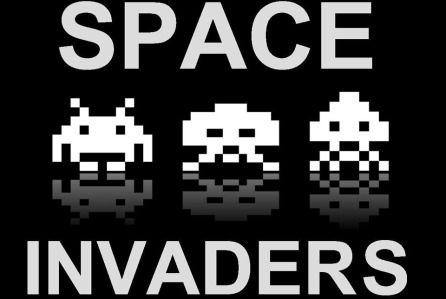
\includegraphics[width=60mm]{space-invaders-2.jpg}
		\caption{Space Invaders Poster}
	\end{figure}


    \begin{itemize}
        \item A classic arcade game 
        \item Released in 1978
    \end{itemize}
\end{frame}

\begin{frame}
The game screen looks like this:
\begin{figure}[ht!]
\centering
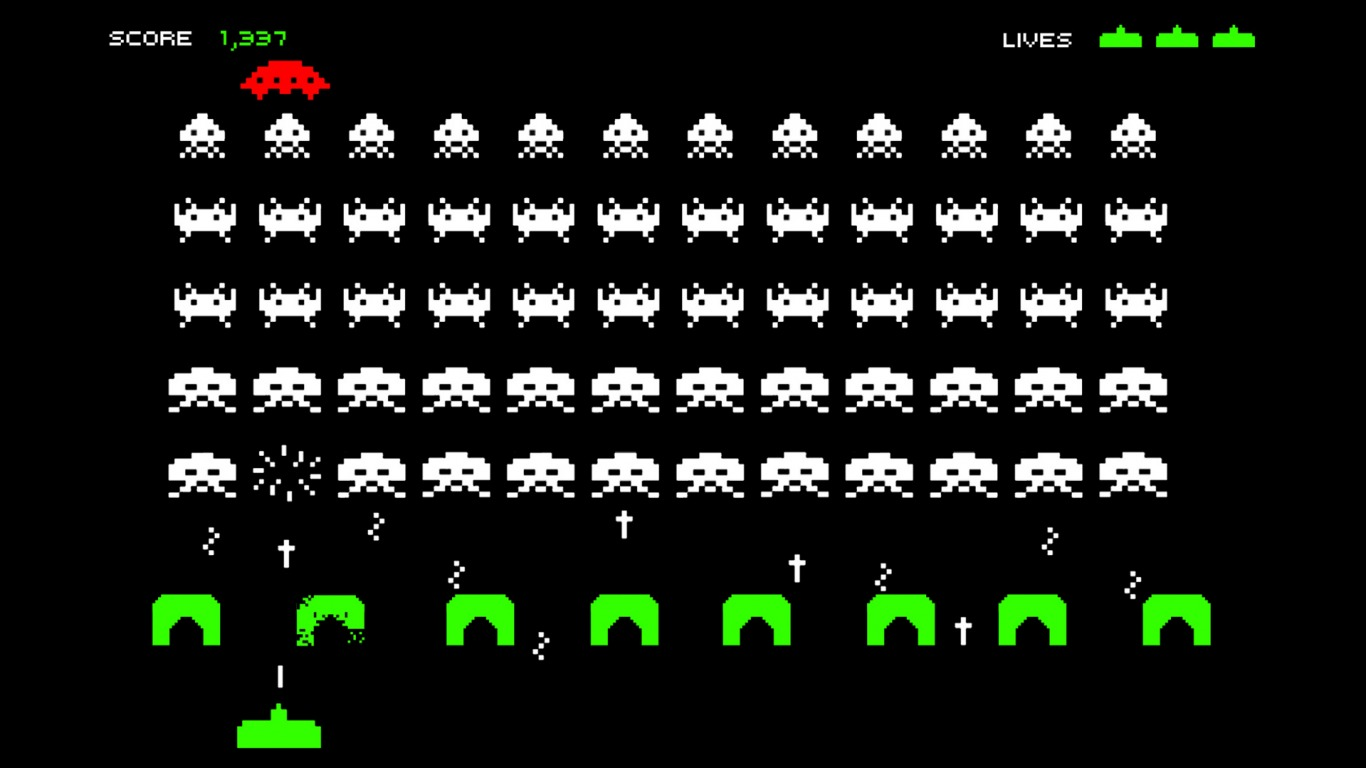
\includegraphics[width=110mm]{space_invaders_screen.jpg}
\caption{Space Invaders's game screen}
\end{figure}
\end{frame}

\begin{frame}
Enemies:
	\begin{figure}[ht!]
	\centering
	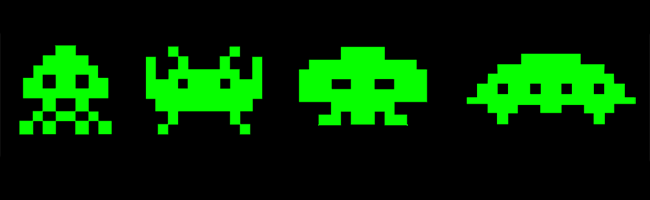
\includegraphics[width=80mm]{basic_enemies.png}
	\caption{Basic Enemies}
	\end{figure}
From Left:
	\begin{itemize}
		\item Large Invader
		\item Medium Invader
		\item Small Invader
		\item The UFO/Mothership
	\end{itemize}
\end{frame}

\begin{frame}
List of things to use:

\begin{figure}[!tbp]
  \centering
  \begin{minipage}[b]{0.4\textwidth}
    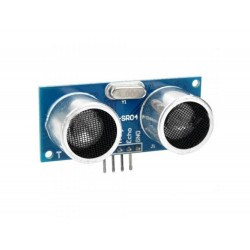
\includegraphics[width=.5\textwidth]{sonar_sensor.jpg}
    \caption{Sonar Sensor}
  \end{minipage}
  \hfill
  \begin{minipage}[b]{0.4\textwidth}
    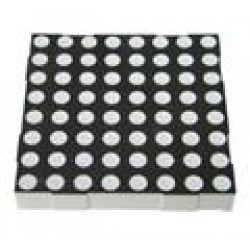
\includegraphics[width=.5\textwidth]{dot_matrix.jpg}
    \caption{Dot Matrix}
  \end{minipage}
  \end{figure}
  \begin{figure}
    \centering
  \begin{minipage}[b]{0.4\textwidth}
    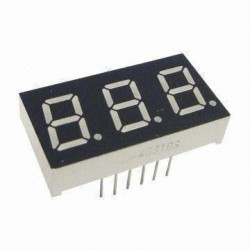
\includegraphics[width=.5\textwidth]{seven_segment.jpg}
    \caption{Seven Segment Display}
  \end{minipage}
    \hfill
  \begin{minipage}[b]{0.4\textwidth}
    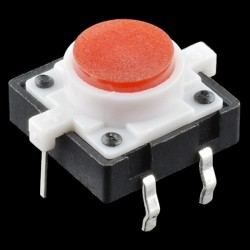
\includegraphics[width=.5\textwidth]{push_button.jpg}
    \caption{Push Button}
  \end{minipage}
\end{figure}

\end{frame}

\begin{frame}

1. LED/Dot Matrix --- For the game display

2. 1/2 Buttons --- To shoot using player and star/stop game

3. A sonar sensor --- To move the player left-right direction

4. 7-segment display --- To show score

\end{frame}


\begin{frame}%%     1
\begin{center}
\Huge Thank You!
\end{center}
\end{frame}


\end{document}